\documentclass[tikz,border=10pt]{standalone}
\usepackage{amsmath}
\usepackage[T1]{fontenc}
\usepackage{pgfplots}
\pgfplotsset{compat=1.18}
\usepgfplotslibrary{groupplots}
\usetikzlibrary{arrows.meta}

\definecolor{cblue}{RGB}{56,110,190}
\definecolor{corange}{RGB}{225,140,45}
\definecolor{cgreen}{RGB}{60,150,70}
\definecolor{cpurple}{RGB}{130,90,200}
\definecolor{cteal}{RGB}{30,150,150}
\definecolor{cred}{RGB}{205,70,70}
\definecolor{cnavy}{RGB}{20,40,80}

\begin{document}
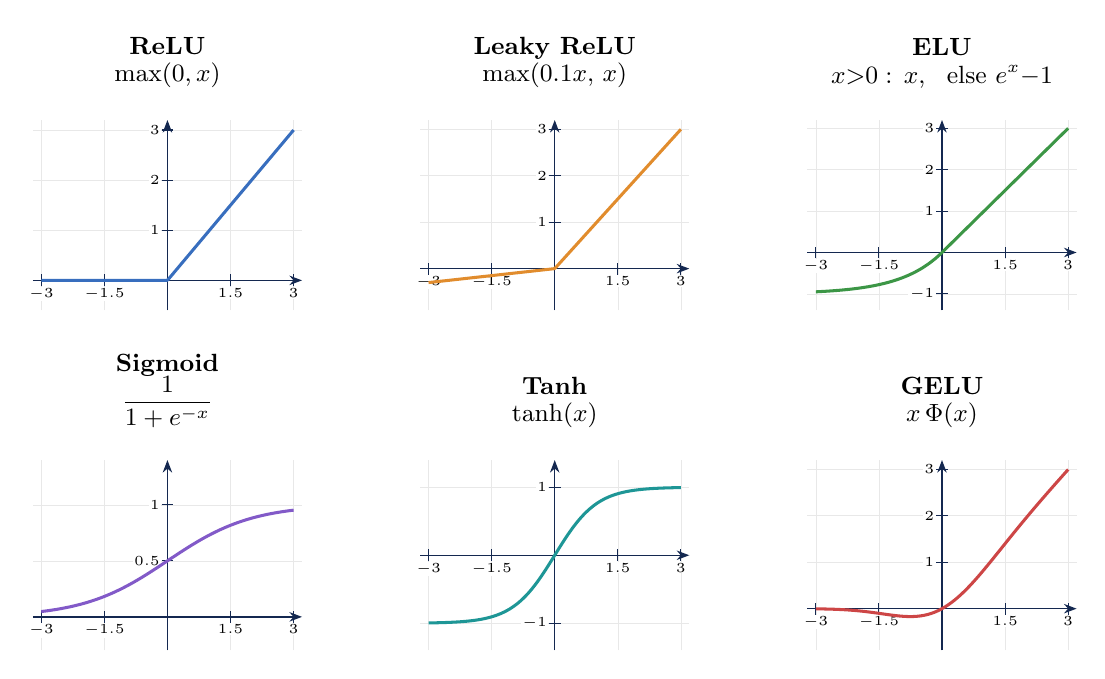
\begin{tikzpicture}
\begin{groupplot}[
  group style={group size=3 by 2, horizontal sep=1.5cm, vertical sep=1.9cm},
  width=5.0cm, height=4.0cm,
  axis lines=middle,
  axis line style={cnavy, -{Stealth[length=1.6mm]}, line width=0.5pt},
  xmin=-3.2, xmax=3.2,
  xtick={-3,-1.5,1.5,3}, xticklabel style={font=\tiny, fill=white, inner sep=0.5pt},
  ytick={-1,1,2,3}, yticklabel style={font=\tiny, fill=white, inner sep=0.5pt},
  tick style={cnavy, line width=0.4pt},
  every axis plot/.append style={line width=1.1pt, samples=200},
  title style={align=center, font=\small, yshift=2pt},
  grid=major, grid style={gray!18, line width=0.2pt},
  clip=false,
]

% ReLU
\nextgroupplot[ymin=-0.6, ymax=3.2, title={\textbf{ReLU}\\[-1pt]$\max(0,x)$}]
  \addplot[cblue, domain=-3:3] {max(0,x)};

% Leaky ReLU
\nextgroupplot[ymin=-0.9, ymax=3.2, title={\textbf{Leaky ReLU}\\[-1pt]$\max(0.1x,\,x)$}]
  \addplot[corange, domain=-3:3] {max(0.1*x,x)};

% ELU
\nextgroupplot[ymin=-1.4, ymax=3.2, title={\textbf{ELU}\\[-1pt]$x{>}0:\,x,\ \ \mathrm{else}\ e^{x}{-}1$}]
  \addplot[cgreen, domain=-3:3] {x>0 ? x : exp(x)-1};

% Sigmoid
\nextgroupplot[ymin=-0.3, ymax=1.4, ytick={0.5,1}, title={\textbf{Sigmoid}\\[-1pt]$\dfrac{1}{1+e^{-x}}$}]
  \addplot[cpurple, domain=-3:3] {1/(1+exp(-x))};

% Tanh
\nextgroupplot[ymin=-1.4, ymax=1.4, ytick={-1,1}, title={\textbf{Tanh}\\[-1pt]$\tanh(x)$}]
  \addplot[cteal, domain=-3:3] {tanh(x)};

% GELU
\nextgroupplot[ymin=-0.9, ymax=3.2, title={\textbf{GELU}\\[-1pt]$x\,\Phi(x)$}]
  \addplot[cred, domain=-3:3] {0.5*x*(1+tanh(0.7978845608*(x+0.044715*x^3)))};

\end{groupplot}
\end{tikzpicture}
\end{document}
